\section{从零做一次}

这一节不采集，只用一张现成的表格走完整条链：上传、分析、出图、看数据、找文件。全程十分钟，不需要登录任何平台。

\subsection{第一步\quad 新建并命名}

菜单条点“\texttt{新建}”，画布清空，状态栏节点数为零。节点库点“\texttt{工作流命名}”，它落在画布中央。
打开设置，在“\texttt{工作流名称}”里写“\texttt{示例 评论情感}”。运行记录和日志以后就用这个名字。

\subsection{第二步\quad 准备表格}

任意一张两列的 CSV，一列分类，一列文本。这一节用二十来条餐厅评论，列名是“\texttt{城市}”与“\texttt{评论}”。
第一行必须是表头，编码用 UTF-8。表格不必大，二十行能看出结果，真实项目几千行流程一样。

\subsection{第三步\quad 上传}

节点库点“\texttt{上传文件}”，放在命名节点右边，打开设置。

\begin{enumerate}
\item 点“\texttt{选择文件}”，挑刚才那张 CSV。
\item 传完面板写文件名、列数、行数，并列出识别到的列名。
\item 文本列选“\texttt{评论}”，下游据此知道读哪一列。
\end{enumerate}

Excel 一次只读一张工作表，多张非空的表会拒绝并列出表名。

\subsection{第四步\quad 分析}

节点库点“\texttt{处理}”，接在上传右边，打开设置。

\begin{enumerate}
\item 操作选“\texttt{情感极性}”，输出标签与零到一的分数。
\item 文本列填“\texttt{评论}”。
\item 分析模式选 \texttt{SnowNLP}，不联网、不占显存。
\item 两个阈值保持默认：正面零点六，负面零点四，中间算中性。
\end{enumerate}

面板底部点“\texttt{预览数据}”，先确认列没选错再往下走。

\subsection{第五步\quad 可视化}

节点库点“\texttt{可视化}”，接在分析节点右边。

\begin{enumerate}
\item 图表类型选“\texttt{柱状图}”，渲染引擎保持 \texttt{ECharts}。
\item 横轴字段选 \texttt{sentiment}，也就是上一步写出的标签列。
\item 聚合方式选“\texttt{计数}”，值字段留空。
\item 图表标题写“\texttt{各情感倾向的评论数}”。
\end{enumerate}

“\texttt{生成 LaTeX 图}”与“\texttt{生成 LaTeX 三线表}”默认勾着，跑完导出目录会多一份可编译的图源。

\subsection{第六步\quad 连线}

三个节点从左到右摆好，用右侧圆点接到下一个节点左侧圆点。命名节点也要连到上传节点，否则运行前会提示它没有下游。

\begin{figure}[H]\centering
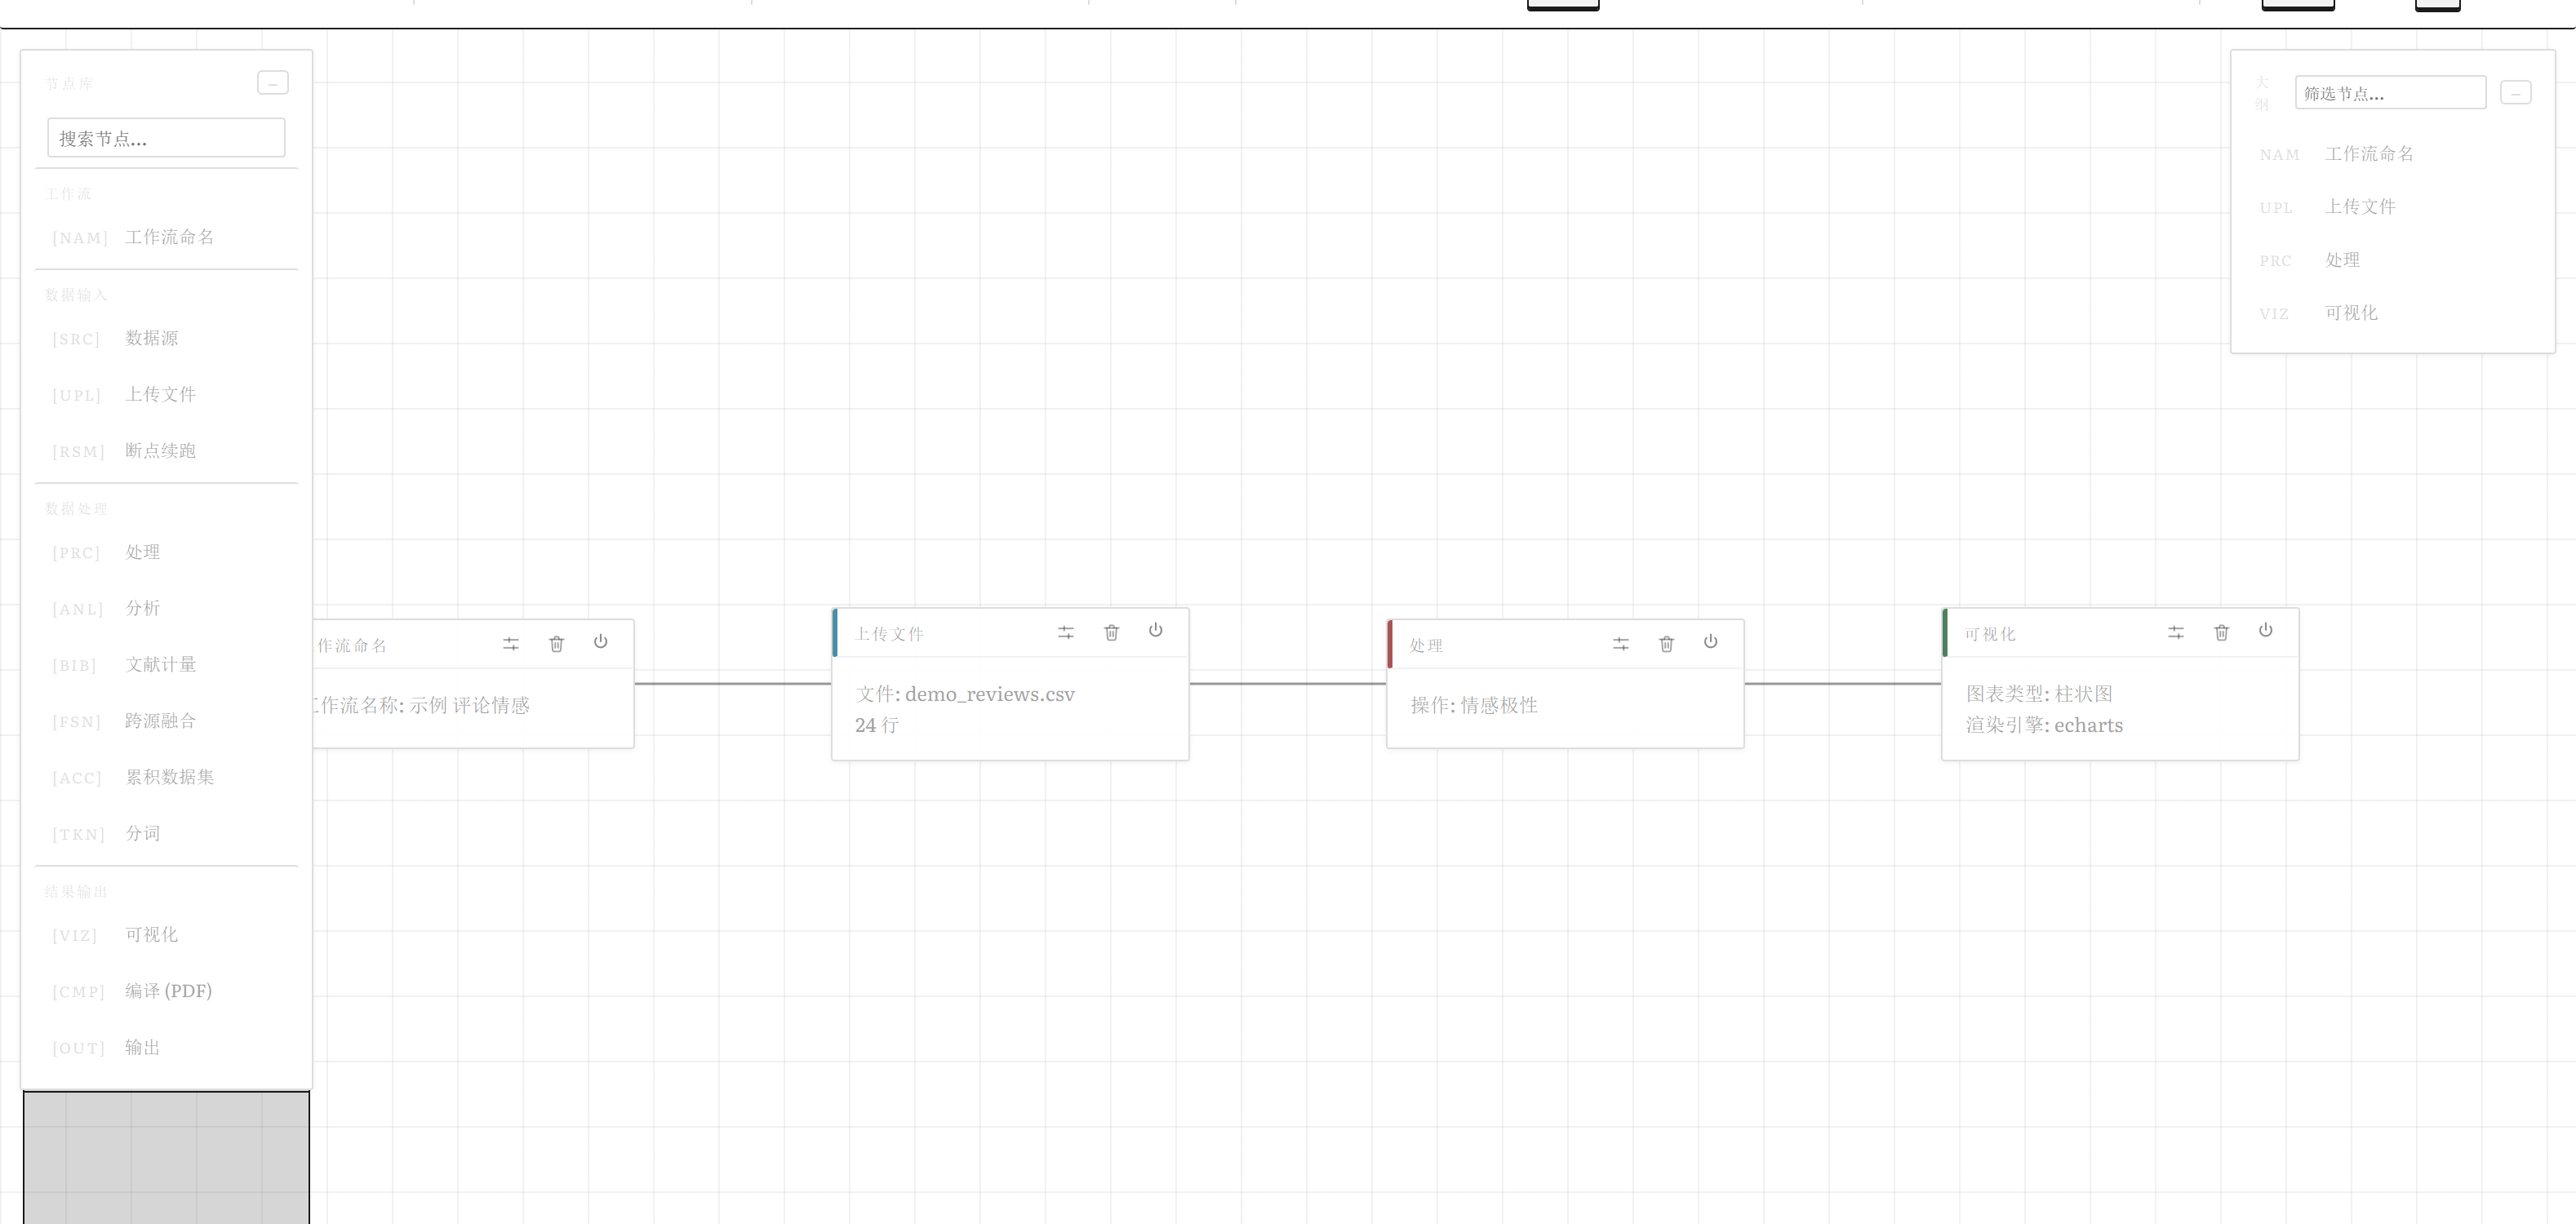
\includegraphics[width=0.9\textwidth]{demo-canvas.png}
\caption{最小的一条工作流：命名、上传、分析、可视化}
\label{fig:demo-canvas}
\end{figure}

\subsection{第七步\quad 保存}

菜单条点“\texttt{保存}”，起名“\texttt{示例-评论情感}”。保存的是画布本身：节点位置、参数、连线、视角。
数据集不存进工作流，工作流只记它的编号，换机器时数据目录要一起搬。

\subsection{第八步\quad 执行}

点“\texttt{执行}”。控制台先写发现了几个节点，再逐个写正在执行哪个、完成几个。二十多行数据几秒钟跑完。
分析节点会打印实际用的模式，可视化节点会打印画了多少行、生成了哪些文件，最后一行是运行结束与完成节点数。

\subsection{第九步\quad 看图}

回到可视化节点，点设置底部的“\texttt{预览图表}”。图在浮层里出现，顶上四个按钮分别是全屏、存为图片、存为 SVG、关闭；
底部还能复制或下载 LaTeX 图源、把图编译成 PDF、复制或下载三线表。

\begin{figure}[H]\centering
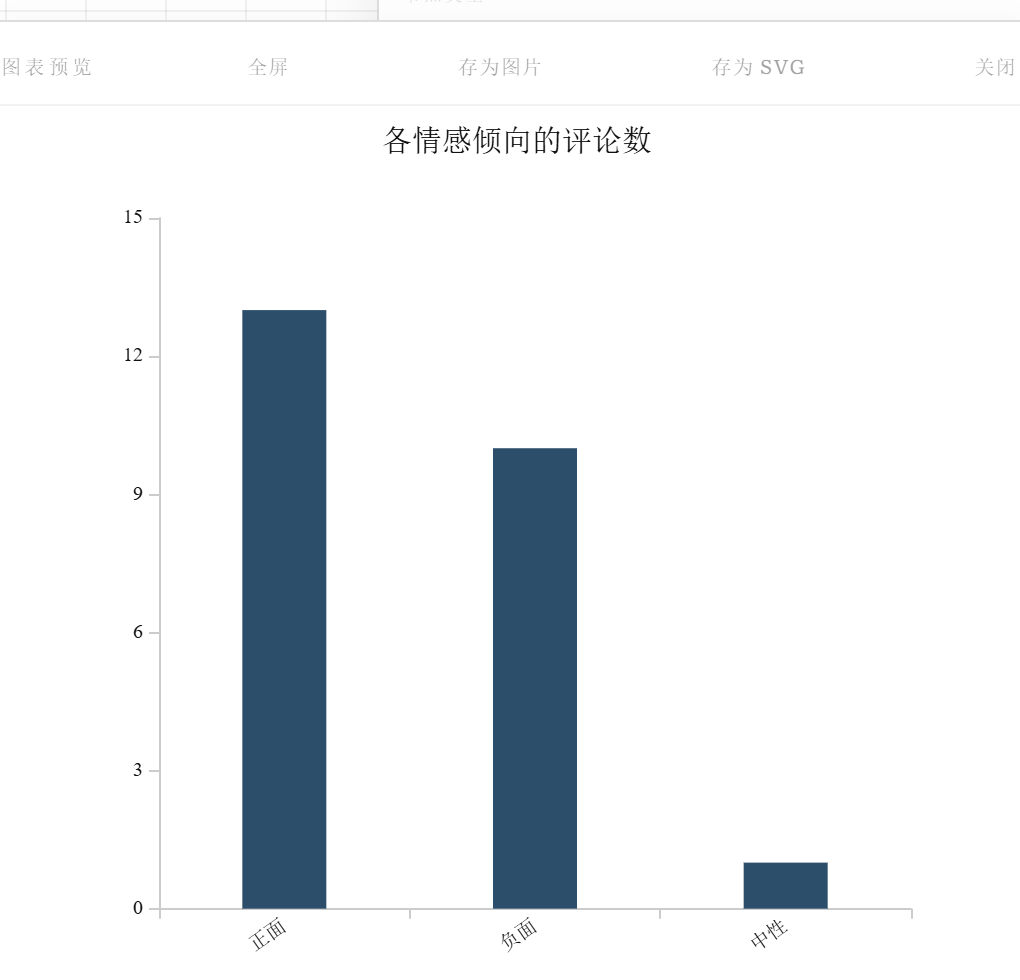
\includegraphics[width=0.72\textwidth]{demo-chart.png}
\caption{预览图表：论文样式的柱状图，正面十三、负面十、中性一}
\label{fig:demo-chart}
\end{figure}

坐标轴只留左边与下面两条，网格很浅，柱条是直角，分类多时横轴自动斜排，每一格都显示，不为避让丢标签。

\subsection{第十步\quad 翻数据}

回到分析节点，点“\texttt{预览数据}”。表头写着行数与列数，底部能翻页，分析结果就在原文右边多出的两列里。

\begin{figure}[H]\centering
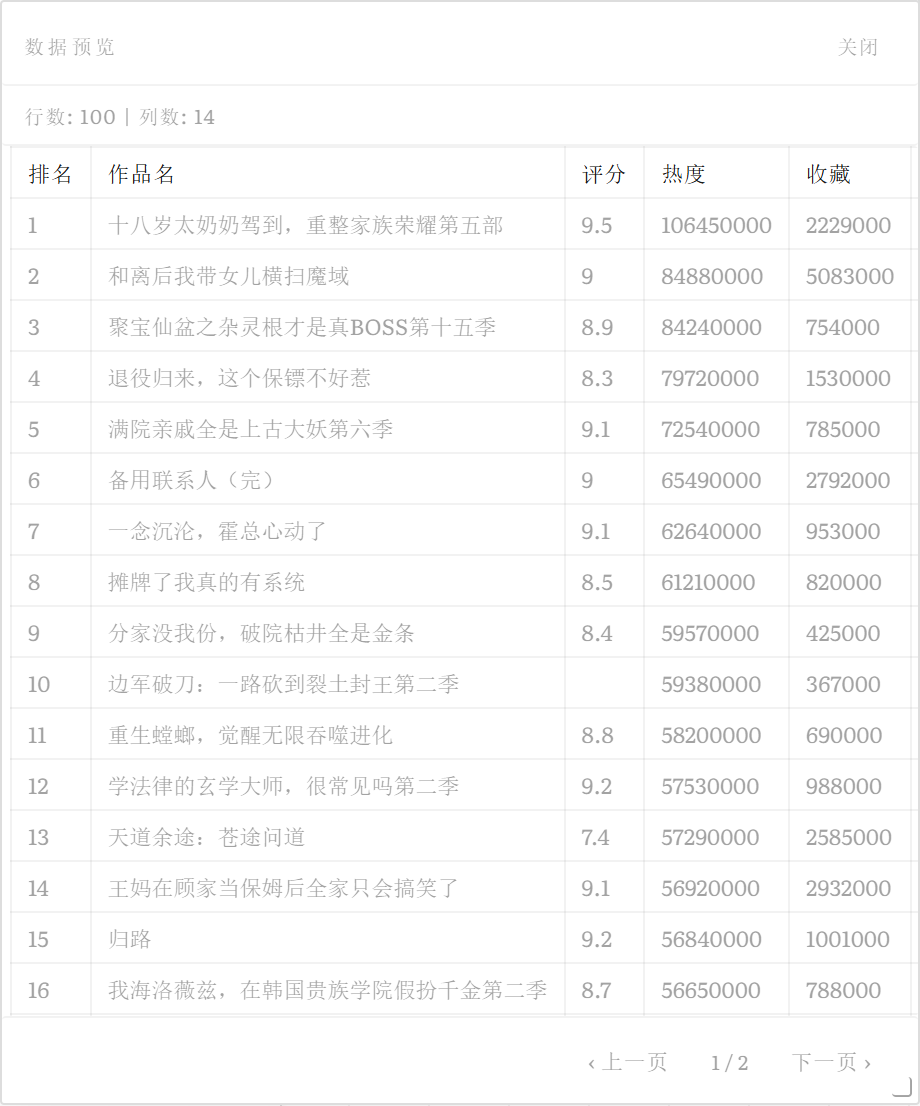
\includegraphics[width=0.72\textwidth]{data-preview.png}
\caption{数据预览：行数、列数、翻页，任何一步都能这样翻}
\label{fig:data-preview}
\end{figure}

\subsection{第十一步\quad 找文件与查记录}

底部点“\texttt{导出产物}”，这次运行写下的文件都在：图表的 PNG、LaTeX 图源、三线表。每一行能下载、删除、复制路径。

\begin{figure}[H]\centering
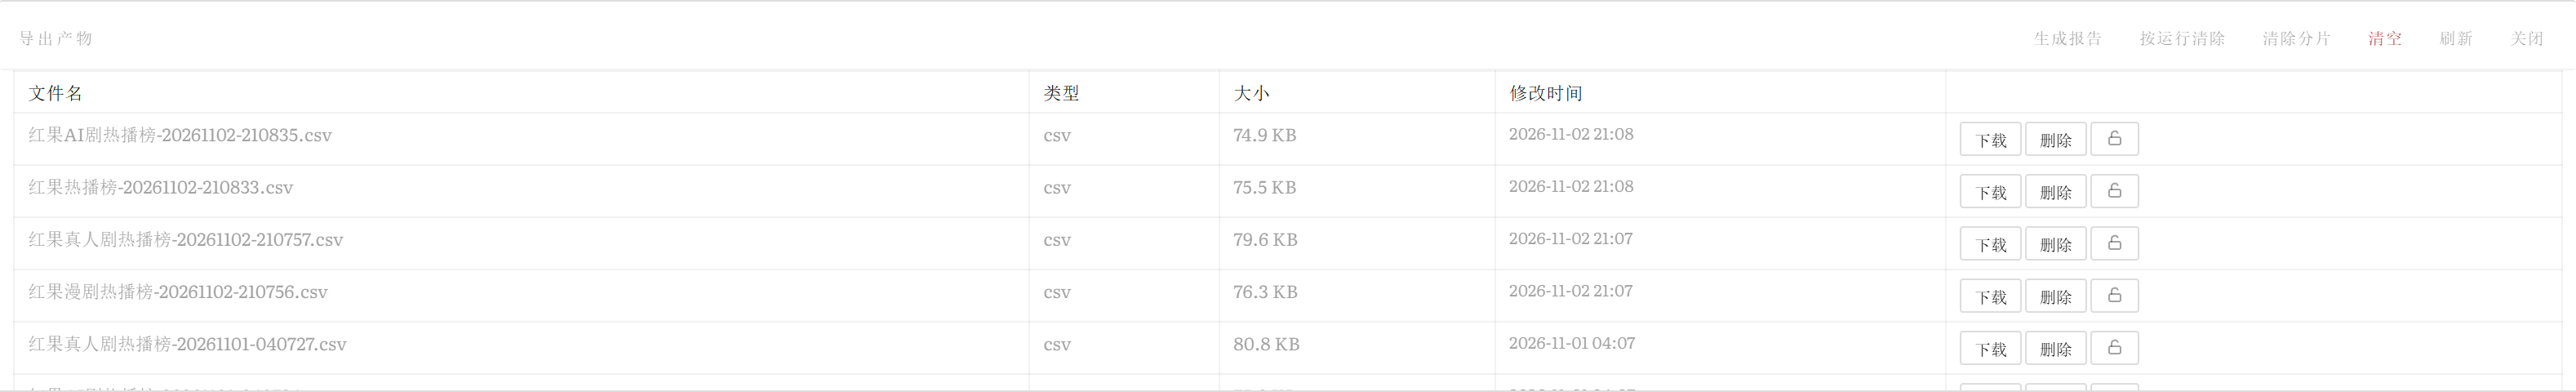
\includegraphics[width=0.96\textwidth]{exports-panel.png}
\caption{导出产物，按运行归档}
\label{fig:exports-panel}
\end{figure}

底部点“\texttt{运行记录}”，这一行写着状态、节点数、行数、开始时间与耗时。右边的按钮能载入这次结果、打开完整日志、生成报告、删除记录。

到这里，建画布、填参数、连线、保存、运行、看图、翻数据、找文件都走了一遍。后面的复杂工作流都是在这几步上叠功能。
